% Created 2014-11-25 mar 17:41
\documentclass[xcolor={usenames,svgnames,dvipsnames}]{beamer}
\usepackage[utf8]{inputenc}
\usepackage[T1]{fontenc}
\usepackage{fixltx2e}
\usepackage{graphicx}
\usepackage{longtable}
\usepackage{float}
\usepackage{wrapfig}
\usepackage{rotating}
\usepackage[normalem]{ulem}
\usepackage{amsmath}
\usepackage{textcomp}
\usepackage{marvosym}
\usepackage{wasysym}
\usepackage{amssymb}
\usepackage{hyperref}
\tolerance=1000
\usepackage{color}
\usepackage{listings}
\AtBeginSection[]{\begin{frame}[plain]\tableofcontents[currentsection,hideallsubsections]\end{frame}}
\lstset{keywordstyle=\color{blue}, commentstyle=\color{gray!90}, basicstyle=\ttfamily\small, columns=fullflexible, breaklines=true,linewidth=\textwidth, backgroundcolor=\color{gray!23}, basewidth={0.5em,0.4em}, literate={á}{{\'a}}1 {ñ}{{\~n}}1 {é}{{\'e}}1 {ó}{{\'o}}1 {º}{{\textordmasculine}}1}
\usepackage{mathpazo}
\hypersetup{colorlinks=true, linkcolor=Blue, urlcolor=Blue}
\usepackage{fancyvrb}
\DefineVerbatimEnvironment{verbatim}{Verbatim}{boxwidth=\textwidth, fontsize=\tiny, formatcom = {\color{black!70}}}
\usepackage{animate}
\usetheme{Goettingen}
\usecolortheme{rose}
\usefonttheme{serif}
\author{Oscar Perpiñán Lamigueiro y Marcelo Pinho Almeida}
\date{24 de Octubre de 2014}
\title{\texttt{meteoForecast}: predicciones meteorológicas de modelos NWP en \texttt{R}}
\hypersetup{
  pdfkeywords={},
  pdfsubject={},
  pdfcreator={Emacs 24.4.1 (Org mode 8.2.7c)}}
\begin{document}

\maketitle

\section{Introducción}
\label{sec-1}

\begin{frame}[fragile,label=sec-1-1]{\texttt{meteoForecast}}
 \begin{block}{¿Qué es?}
\texttt{meteoForecast} es un paquete que permite obtener predicciones de
modelos numéricos meteorológicos producidos por diferentes servicios
en formato raster o como series temporales.
\end{block}

\begin{block}{Marco de trabajo}
El desarrollo de este paquete se enmarca dentro del proyecto europeo
\href{http://www.pvcrops.eu/project-deliverables}{PVCROPS}.
\end{block}
\end{frame}

\begin{frame}[label=sec-1-2]{Servicios disponibles}
\begin{columns}
\begin{column}{0.32\textwidth}

\begin{itemize}
\item \href{http://www.emc.ncep.noaa.gov/index.php?branch=GFS}{GFS}
\item \href{http://www.meteogalicia.es/web/modelos/threddsIndex.action}{MeteoGalicia}
\item \href{https://openmeteoforecast.org/}{OpenMeteo}
\item \href{http://www.ncdc.noaa.gov/data-access/model-data/model-datasets/north-american-mesoscale-forecast-system-nam}{NAM}
\item \href{http://www.ncdc.noaa.gov/data-access/model-data/model-datasets/rapid-refresh-rap}{RAP}
\end{itemize}
\end{column}
\begin{column}{0.7\textwidth}
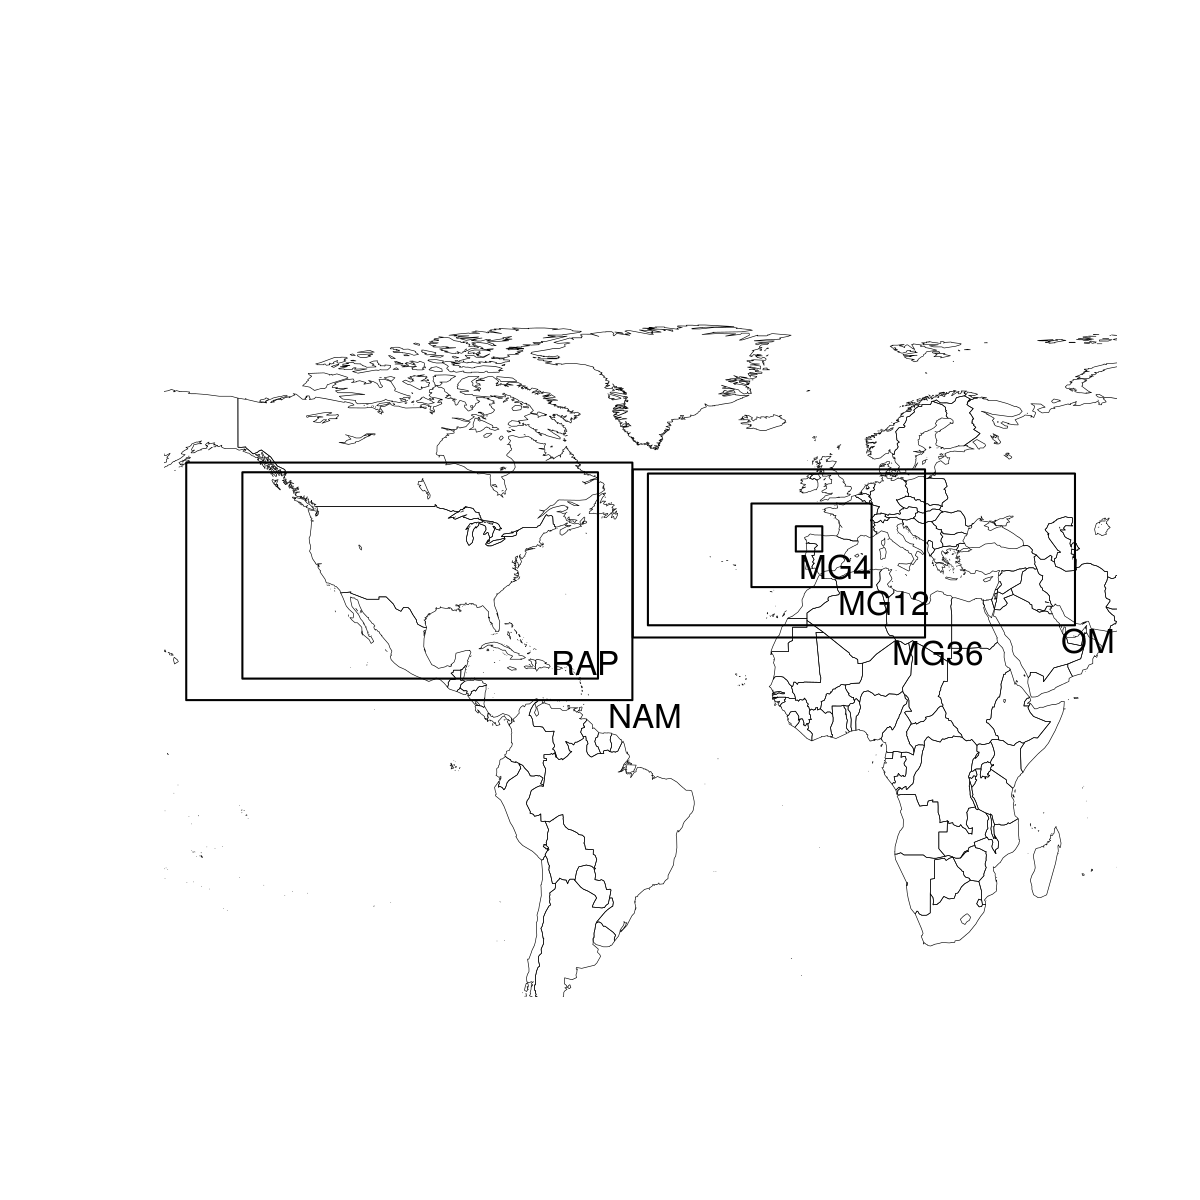
\includegraphics[width=.9\linewidth]{figs/mapaServices.png}
\end{column}
\end{columns}
\end{frame}

\begin{frame}[fragile,label=sec-1-3]{Instalación}
 \begin{itemize}
\item La versión de desarrollo está en GitHub:
\end{itemize}
\lstset{language=R,label= ,caption= ,numbers=none}
\begin{lstlisting}
    install.packages("devtools")
    devtools::install_github("oscarperpinan/meteoForecast")
\end{lstlisting}

\begin{itemize}
\item La versión estable está publicada en \href{http://cran.r-project.org/web/packages/meteoForecast/}{CRAN}:

\lstset{language=R,label= ,caption= ,numbers=none}
\begin{lstlisting}
   install.packages('meteoForecast')
\end{lstlisting}

\item Empezamos
\end{itemize}
\lstset{language=R,label= ,caption= ,numbers=none}
\begin{lstlisting}
  library(meteoForecast)
\end{lstlisting}
\end{frame}


\section{Primeros pasos}
\label{sec-2}

\begin{frame}[fragile,label=sec-2-1]{Variables}
 \begin{itemize}
\item Cada servicio proporciona un conjunto diferente de variables con sus
propios nombres.
\item Su nombre y descripción están disponibles en \texttt{varsMG}, \texttt{varsGFS},
etc.
\end{itemize}
\lstset{language=R,label= ,caption= ,numbers=none}
\begin{lstlisting}
data(varsMG)
\end{lstlisting}
\begin{itemize}
\item \texttt{grepVar} facilita la tarea de buscar la variable que interesa:
\end{itemize}

\lstset{language=R,label= ,caption= ,numbers=none}
\begin{lstlisting}
grepVar('cloud', service = 'gfs')
\end{lstlisting}

\begin{verbatim}
 [1] "Temperature_low_cloud_top"           "Pressure_middle_cloud_top"          
 [3] "Temperature_middle_cloud_top"        "Total_cloud_cover_middle_cloud"     
 [5] "Cloud_Work_Function"                 "Pressure_low_cloud_bottom"          
 [7] "Pressure_convective_cloud_top"       "Pressure_convective_cloud_bottom"   
 [9] "Total_cloud_cover_high_cloud"        "Total_cloud_cover"                  
[11] "Pressure_low_cloud_top"              "Pressure_high_cloud_top"            
[13] "Pressure_middle_cloud_bottom"        "Cloud_mixing_ratio"                 
[15] "Pressure_high_cloud_bottom"          "Total_cloud_cover_convective_cloud" 
[17] "Cloud_water"                         "Total_cloud_cover_entire_atmosphere"
[19] "Total_cloud_cover_low_cloud"         "Temperature_high_cloud_top"
\end{verbatim}
\end{frame}


\begin{frame}[fragile,label=sec-2-2]{Servicios}
 \begin{itemize}
\item Cada función admite un argumento \texttt{service} para elegir el servicio.
\item Al cargar el paquete el servicio por defecto es MeteoGalicia.
\end{itemize}
\lstset{language=R,label= ,caption= ,numbers=none}
\begin{lstlisting}
mfService()
\end{lstlisting}

\begin{verbatim}
[1] "meteogalicia"
\end{verbatim}

\begin{itemize}
\item Se puede cambiar (para una sesión) usando \texttt{mfService} con el nombre
del servicio.
\end{itemize}
\lstset{language=R,label= ,caption= ,numbers=none}
\begin{lstlisting}
mfService('gfs')
\end{lstlisting}

\begin{verbatim}
Option service changed to gfs
\end{verbatim}

\lstset{language=R,label= ,caption= ,numbers=none}
\begin{lstlisting}
mfService('meteogalicia')
\end{lstlisting}

\begin{verbatim}
Option service changed to meteogalicia
\end{verbatim}
\end{frame}

\begin{frame}[fragile,label=sec-2-3]{Información sobre cada servicio}
 \begin{itemize}
\item \texttt{mfProj4} devuelve la proyección (Proj4) de un servicio:
\end{itemize}
\lstset{language=R,label= ,caption= ,numbers=none}
\begin{lstlisting}
mfProj4('nam')
\end{lstlisting}

\begin{verbatim}
[1] "+proj=lcc +lat_1=25 +lat_0=25 +lon_0=-95 +k_0=1 +x_0=0 +y_0=0 +a=6367470.21484375 +b=6367470.21484375 +units=km +no_defs "
\end{verbatim}

\begin{itemize}
\item \texttt{mfExtent} devuelve la extensión de un servicio (usando la clase \texttt{Extent} del paquete \texttt{raster}):
\end{itemize}
\lstset{language=R,label= ,caption= ,numbers=none}
\begin{lstlisting}
mfExtent('meteogalicia', resolution = 36)
\end{lstlisting}

\begin{verbatim}
class       : Extent 
xmin        : -49.18259 
xmax        : 18.789 
ymin        : 24.03791 
ymax        : 56.06608
\end{verbatim}
\end{frame}

\section{NWP para una región: \texttt{getRaster*}}
\label{sec-3}

\begin{frame}[fragile,label=sec-3-1]{\texttt{getRaster}}
 \begin{itemize}
\item \texttt{getRaster} descarga ficheros NetCDF con resultados del modelo NWP
para un región emitidos un día determinado y los acondiciona en un
objeto \texttt{RasterBrick}.
\item La extensión, la resolución temporal, y el horizonte de predicción
dependen de cada servicio.
\end{itemize}

\lstset{language=R,label= ,caption= ,numbers=none}
\begin{lstlisting}
  ## temperature at 2m
  wrf <- getRaster(var = 'temp',
                   day = '2014-01-25',
                   run = '00')
\end{lstlisting}
\end{frame}

\begin{frame}[label=sec-3-2]{}
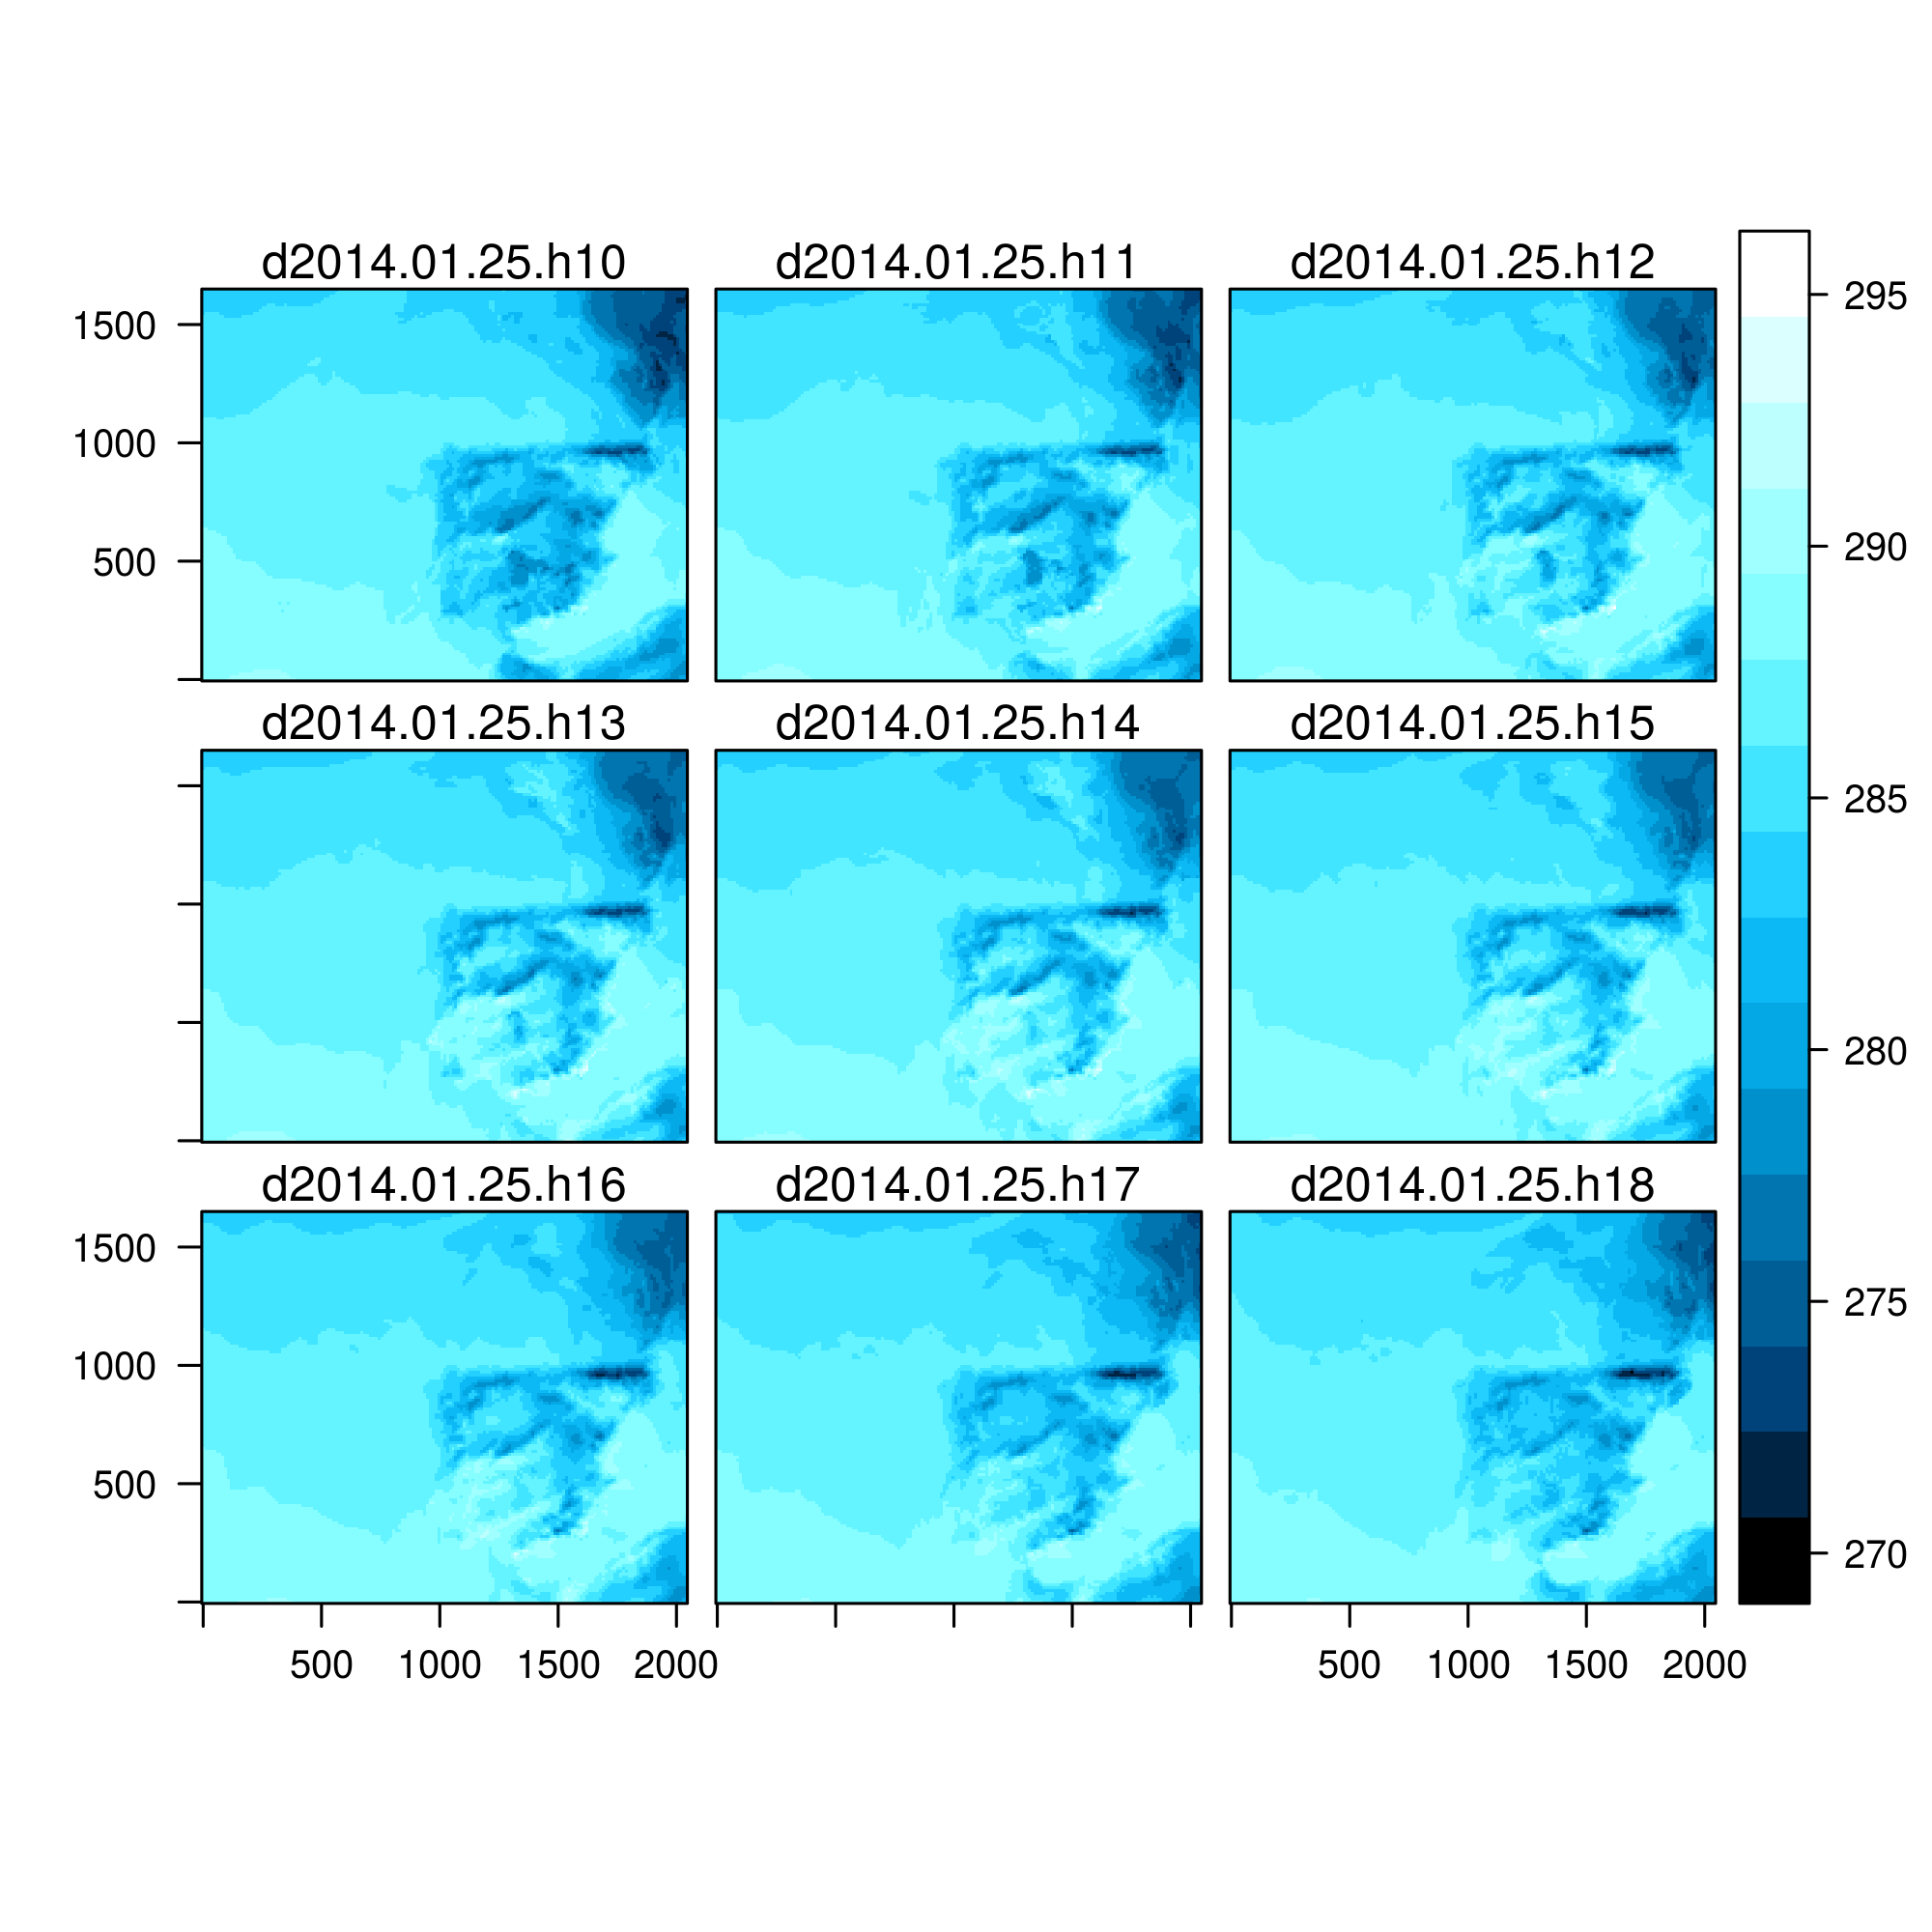
\includegraphics[width=.9\linewidth]{figs/wrf.png}
\end{frame}

\begin{frame}[fragile,label=sec-3-3]{Limitando la región y el periodo temporal}
 \lstset{language=R,label= ,caption= ,numbers=none}
\begin{lstlisting}
cloudNAM <- getRaster('Total_cloud_cover',
                      day = '2014-10-01',
                      box = c(-100, -80, 30, 50),
                      frames = 10,
                      service = 'nam')
\end{lstlisting}

\begin{verbatim}
class       : RasterLayer 
dimensions  : 196, 159, 31164  (nrow, ncol, ncell)
resolution  : 0.1537046, 0.1084714  (x, y)
extent      : -101.1972, -76.75821, 29.35018, 50.61057  (xmin, xmax, ymin, ymax)
coord. ref. : +proj=longlat +datum=WGS84 +ellps=WGS84 +towgs84=0,0,0
\end{verbatim}

\lstset{language=R,label= ,caption= ,numbers=none}
\begin{lstlisting}
getZ(cloudNAM)
\end{lstlisting}

\begin{verbatim}
[1] "2014-10-01 01:00:00 UTC" "2014-10-01 02:00:00 UTC"
[3] "2014-10-01 03:00:00 UTC" "2014-10-01 04:00:00 UTC"
[5] "2014-10-01 05:00:00 UTC" "2014-10-01 06:00:00 UTC"
[7] "2014-10-01 07:00:00 UTC" "2014-10-01 08:00:00 UTC"
[9] "2014-10-01 09:00:00 UTC" "2014-10-01 10:00:00 UTC"
\end{verbatim}
\end{frame}

\begin{frame}[fragile,label=sec-3-4]{\texttt{getRasterDay} y \texttt{getRasterDays}}
 \begin{itemize}
\item \texttt{getRasterDay} y \texttt{getRasterDays} se basan en \texttt{getRaster} para
obtener resultados exclusivamente para un día determinado y una
secuencia de días, respectivamente.
\end{itemize}

\lstset{language=R,label= ,caption= ,numbers=none}
\begin{lstlisting}
  ## cloud cover at low and mid levels
  wrfDays <- getRasterDays(var = 'cft',
                           start = '2014-01-01',
                           end = '2014-01-05',
                           box = c(-2, 35, 2, 40))
\end{lstlisting}

\begin{verbatim}
class       : RasterStack 
dimensions  : 65, 41, 2665, 120  (nrow, ncol, ncell, nlayers)
resolution  : 12, 12  (x, y)
extent      : 1554, 2046, -6, 774  (xmin, xmax, ymin, ymax)
coord. ref. : +proj=lcc +lat_1=43 +lat_2=43 +lat_0=34.82300186157227 +lon_0=-14.10000038146973 +x_0=536402.34 +y_0=-18558.61 +ellps=WGS84 +towgs84=0,0,0,0,0,0,0 +units=km +no_defs 
names       : d2014.01.01.h01, d2014.01.01.h02, d2014.01.01.h03, d2014.01.01.h04, d2014.01.01.h05, d2014.01.01.h06, d2014.01.01.h07, d2014.01.01.h08, d2014.01.01.h09, d2014.01.01.h10, d2014.01.01.h11, d2014.01.01.h12, d2014.01.01.h13, d2014.01.01.h14, d2014.01.01.h15, ... 
min values  :      0.00000000,      0.00000000,      0.00000000,      0.00000000,      0.00000000,      0.00000000,      0.00000000,      0.00000000,      0.00000000,      0.00000000,      0.00000000,      0.00000000,      0.00000000,      0.00000000,      0.00000000, ... 
max values  :       0.6915230,       0.9363602,       1.0209019,       1.0181180,       0.9741192,       1.0097407,       1.0229231,       1.0159433,       1.0287733,       1.0006489,       0.9815325,       0.9944173,       1.0124562,       1.3608389,       2.4704671, ... 
time        : 2014-01-01 01:00:00 - 2014-01-06 00:00:00 (range)
\end{verbatim}
\end{frame}

\begin{frame}[label=sec-3-5]{}
\animategraphics[width=\textwidth, autoplay,loop]{5}{figs/wrfDays}{001}{120}
\end{frame}


\section{NWP para un punto: \texttt{getPoint*}}
\label{sec-4}

\begin{frame}[fragile,label=sec-4-1]{\texttt{getPoint}}
 \begin{itemize}
\item \texttt{getPoint} descarga resultados emitidos un día determinado por un
modelo NWP para un \alert{punto} y los acondiciona como serie temporal
usando la clase \texttt{zoo}.
\end{itemize}

\lstset{language=R,label= ,caption= ,numbers=none}
\begin{lstlisting}
  ## Radiación solar y temperatura
  vars <- getPoint(point = c(0, 40),
                   day = Sys.Date() - 1, 
                   vars = c('swflx', 'temp'))
  attr(vars, 'lat')
  attr(vars, 'lon')
\end{lstlisting}
\end{frame}
\begin{frame}[label=sec-4-2]{}
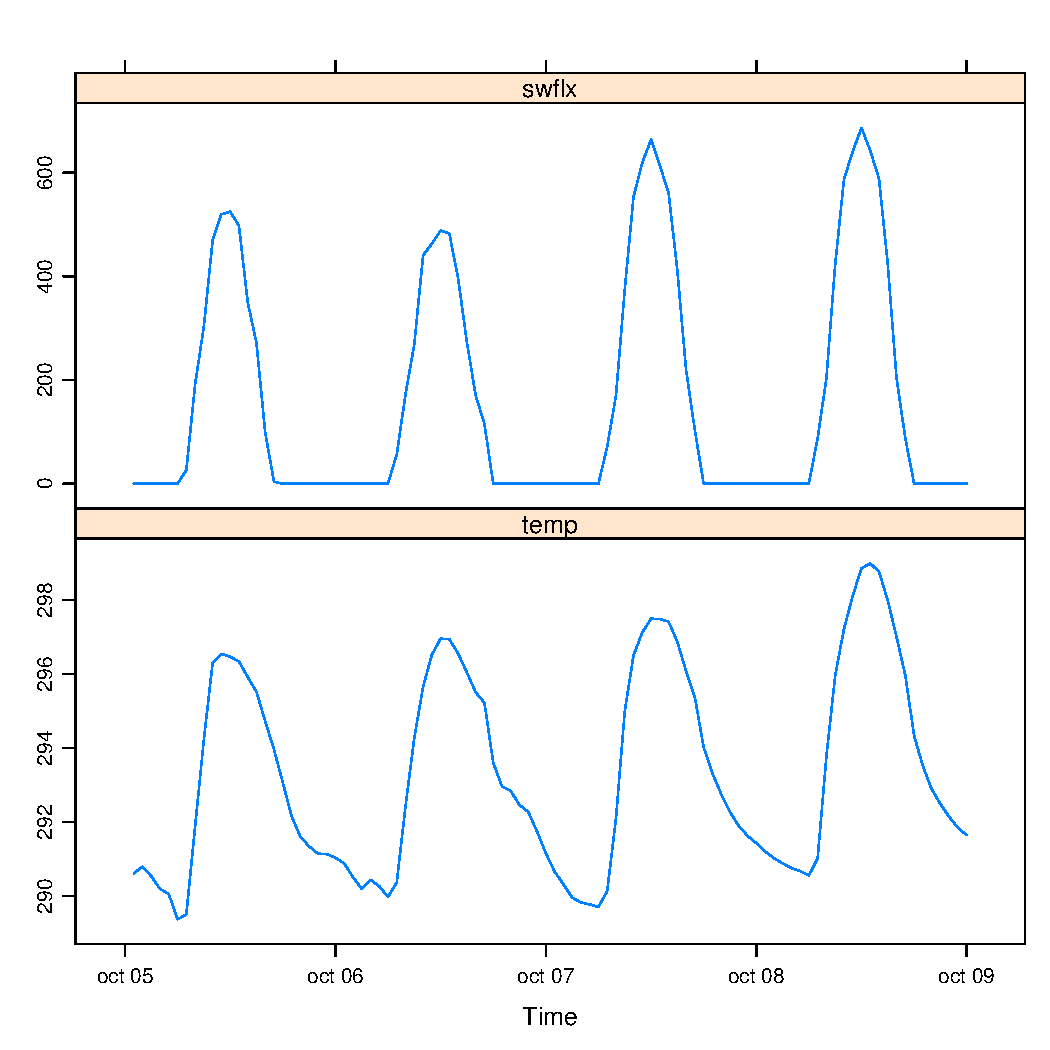
\includegraphics[width=.9\linewidth]{figs/point.pdf}
\end{frame}

\begin{frame}[fragile,label=sec-4-3]{\texttt{getPointDays}}
 \begin{itemize}
\item \texttt{getPointDays} usa \texttt{getPoint} para construir una secuencia de días.
\end{itemize}
\lstset{language=R,label= ,caption= ,numbers=none}
\begin{lstlisting}
  radDays <- getPointDays(point = c(0, 40),
                          var = 'swflx',
                          start = '2013-01-01',
                          end = '2013-01-15')
\end{lstlisting}
\end{frame}

\begin{frame}[label=sec-4-4]{}
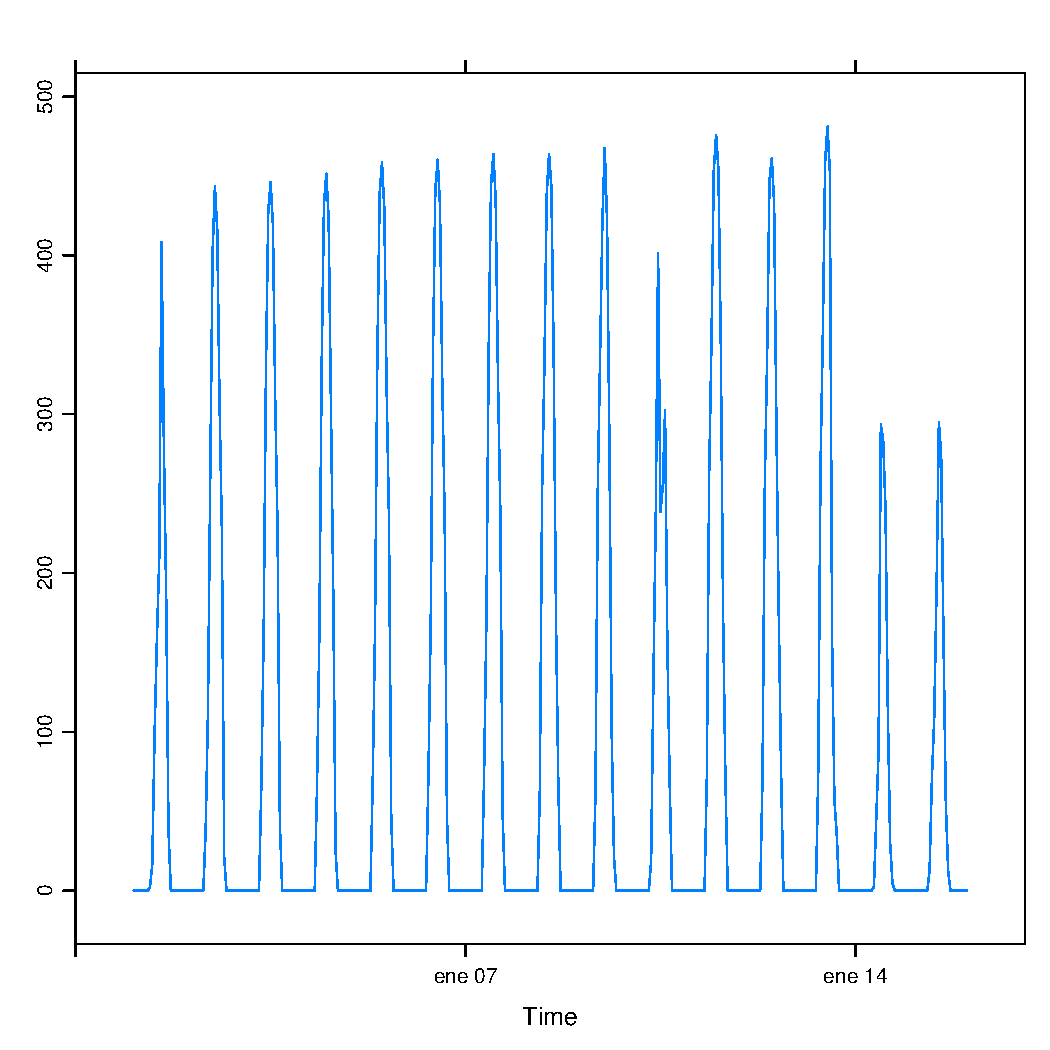
\includegraphics[width=.9\linewidth]{figs/radDays.pdf}
\end{frame}

\begin{frame}[fragile,label=sec-4-5]{\texttt{getPointRuns}}
 \begin{itemize}
\item \texttt{getPointRuns} usa \texttt{getPoint} para producir una serie temporal de
predicciones, donde cada columna indica cuando fue emitida esa
predicción.
\end{itemize}
\lstset{language=R,label= ,caption= ,numbers=none}
\begin{lstlisting}
  ## Variability between runs
  radRuns <- getPointRuns(c(0, 40),
                          var = 'swflx',
                          start = '2013-01-01',
                          end = '2013-01-15')
\end{lstlisting}
\end{frame}

\begin{frame}[label=sec-4-6]{}
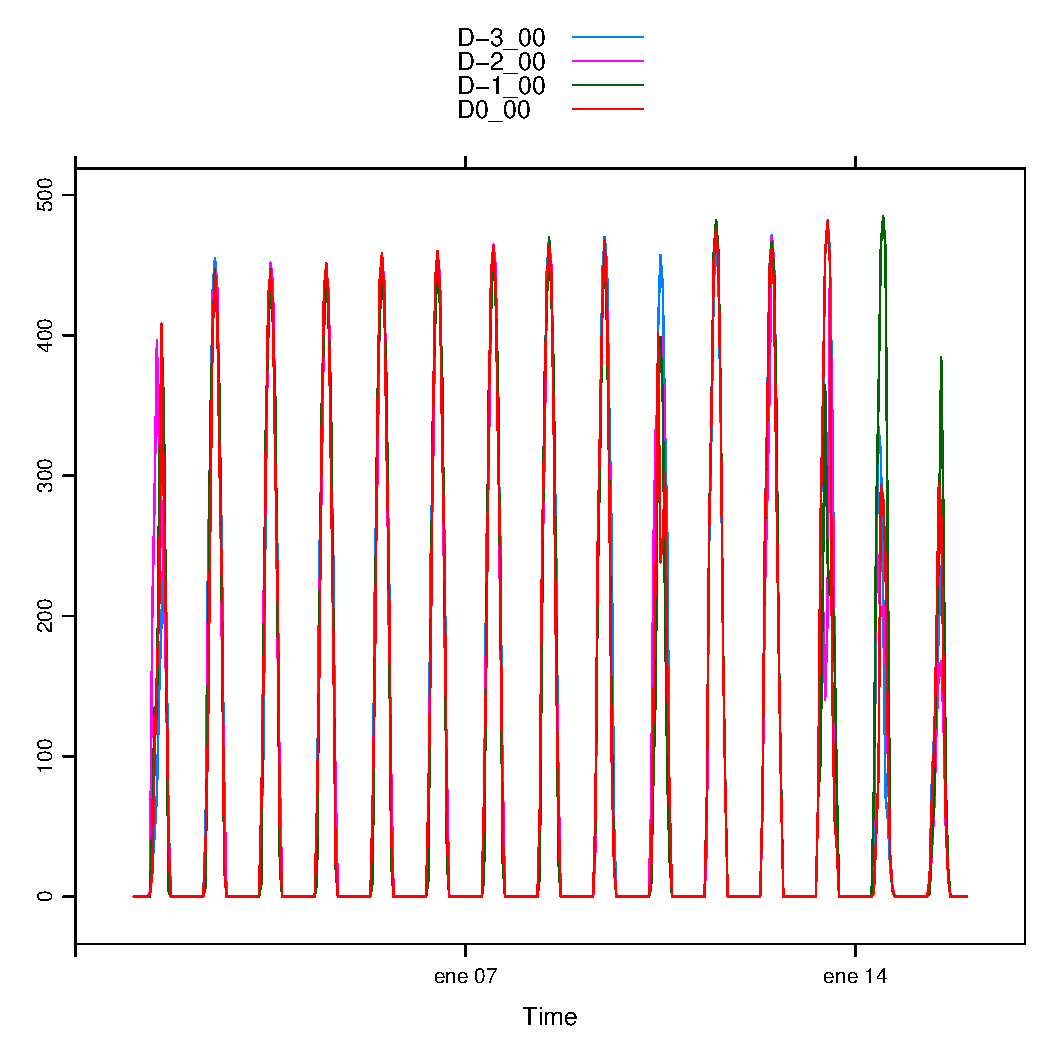
\includegraphics[width=.9\linewidth]{figs/radRuns.pdf}
\end{frame}

\begin{frame}[fragile,label=sec-4-7]{}
 \lstset{language=R,label= ,caption= ,numbers=none}
\begin{lstlisting}
## variability around the average
radAv <- rowMeans(radRuns)
radVar <- sweep(radRuns, 1, radAv)
\end{lstlisting}
\end{frame}

\begin{frame}[label=sec-4-8]{}
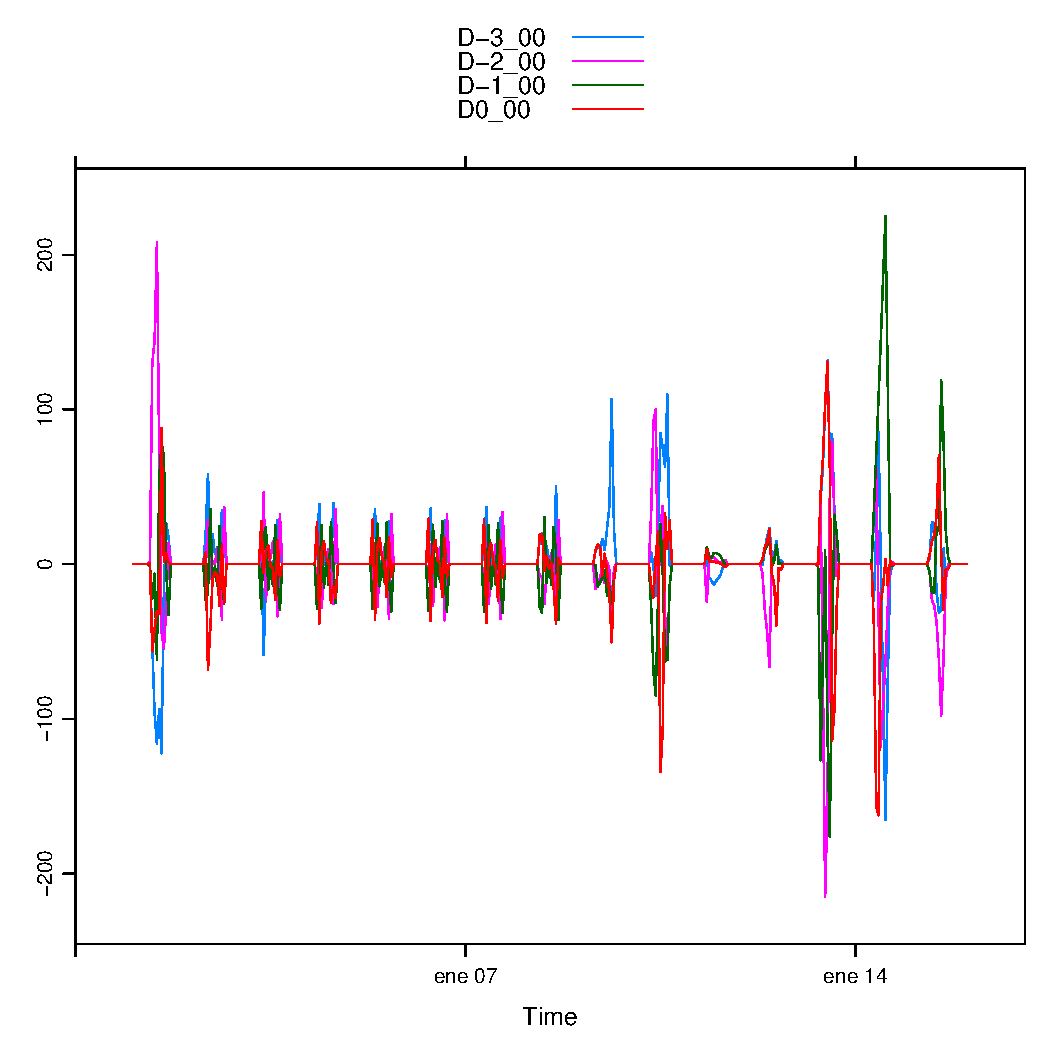
\includegraphics[width=.9\linewidth]{figs/radVar.pdf}
\end{frame}
% Emacs 24.4.1 (Org mode 8.2.7c)
\end{document}